\documentclass[wide,a4paper,titlepage,12pt] {article}
\usepackage{polski}
\usepackage[utf8]{inputenc}
\usepackage{listings}
\usepackage{slashbox}
\usepackage[table]{xcolor}
\usepackage{graphicx,pdflscape}
\usepackage{placeins}


\title{Technologie sieciowe 2}
\author{Tymon Tobolski (181037)\\ Jacek Wieczorek (181043)}

% Title page layout (fold)
\makeatletter
\renewcommand{\maketitle}{
\begin{titlepage}
  \begin{center}
    \vspace*{3cm}
    \LARGE \@title \par
    \vspace{2cm}
    \textit{\small Autor:}\par
    \normalsize \@author\par \normalsize
    \vspace{3cm}
    \textit{\small Prowadzący:}\par
    Dr inż. Andrzej Grzybowski\par
    \vspace{2cm}
    Wydział Elektroniki\\ III rok\\ Pn TN 11.15 - 13.00\par
    \vspace{4cm}
    \small \@date
  \end{center}
\end{titlepage}
}
\makeatother


\begin{document}
\maketitle
  \section{Cel laboratorium}
  \paragraph{}

  \section{Zadania}

  \subsection{Zadanie 1}
  \paragraph{}
  Po podłączeniu wszystkich urządzeń i wejściu się przez przeglądarkę pod adres \textbf{192.168.1.1} ukazało się okno logowania. Domyślna nazwa użytkownika to \textbf{???}, a hasło \textbf{???}.
  W celu ustawienia połączenia z internetem należało wybrać opcję \textbf{Dynamic IP Address (Cable Modem User)}.

  \begin{figure}[h!]
    \begin{center}
      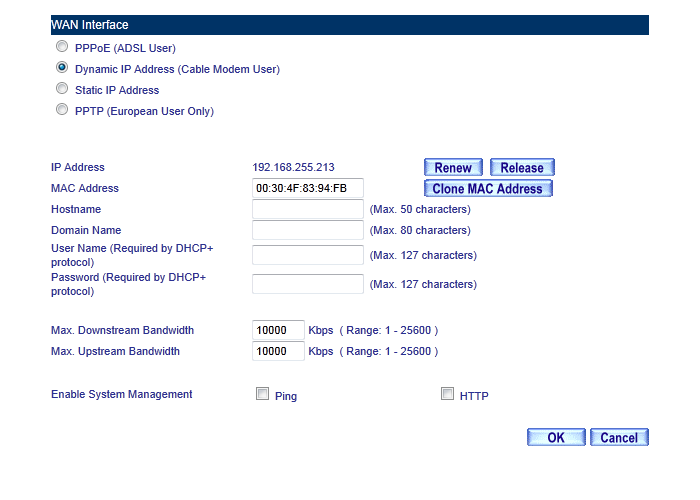
\includegraphics[width=\textwidth]{1.PNG}
    \end{center}
  \end{figure}


  \subsection{Zadanie 2}


  \subsection{Zadanie 3}
  \paragraph{}
  Ustawienie polisy umożliwiającej wyjście do Internetu.
  \begin{figure}[h!]
    \begin{center}
      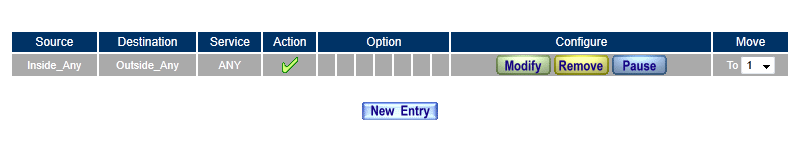
\includegraphics[width=\textwidth]{2.PNG}
    \end{center}
  \end{figure}



  \subsection{Zadanie 4}
  \paragraph{}
  Zdefiniowane adresu 2 komputerów.
  \begin{figure}[h!]
    \begin{center}
      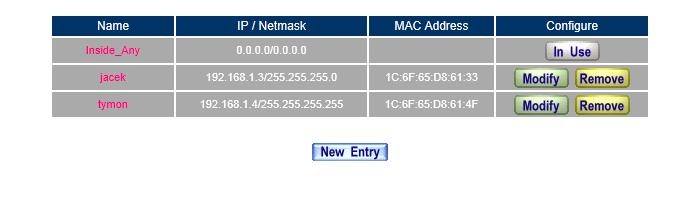
\includegraphics[width=\textwidth]{3.PNG}
    \end{center}
  \end{figure}


  \subsection{Zadanie 5}
  \paragraph{}
  Zdefiniowane reguły QoS.
  \begin{figure}[h!]
    \begin{center}
      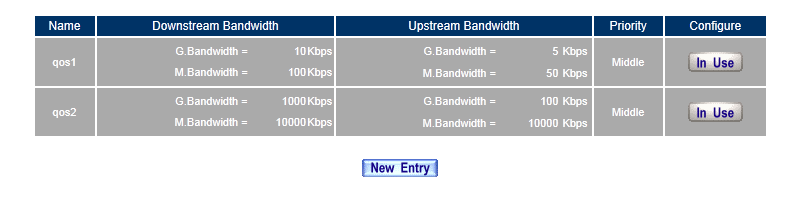
\includegraphics[width=\textwidth]{3_5.PNG}
      \caption{}
    \end{center}
  \end{figure}



  \subsection{Zadanie 6}
  \paragraph{}
  Reguły ograniczające pasmo.

  \begin{figure}[h!]
    \begin{center}
      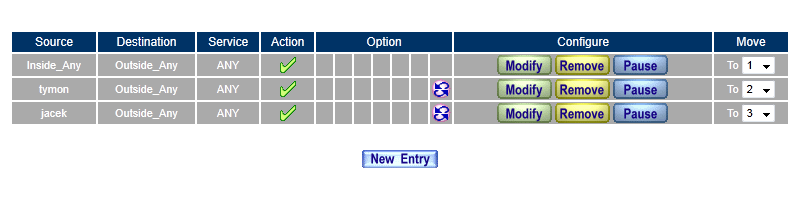
\includegraphics[width=\textwidth]{4.PNG}
    \end{center}
  \end{figure}

  \begin{figure}[h!]
    \begin{center}
      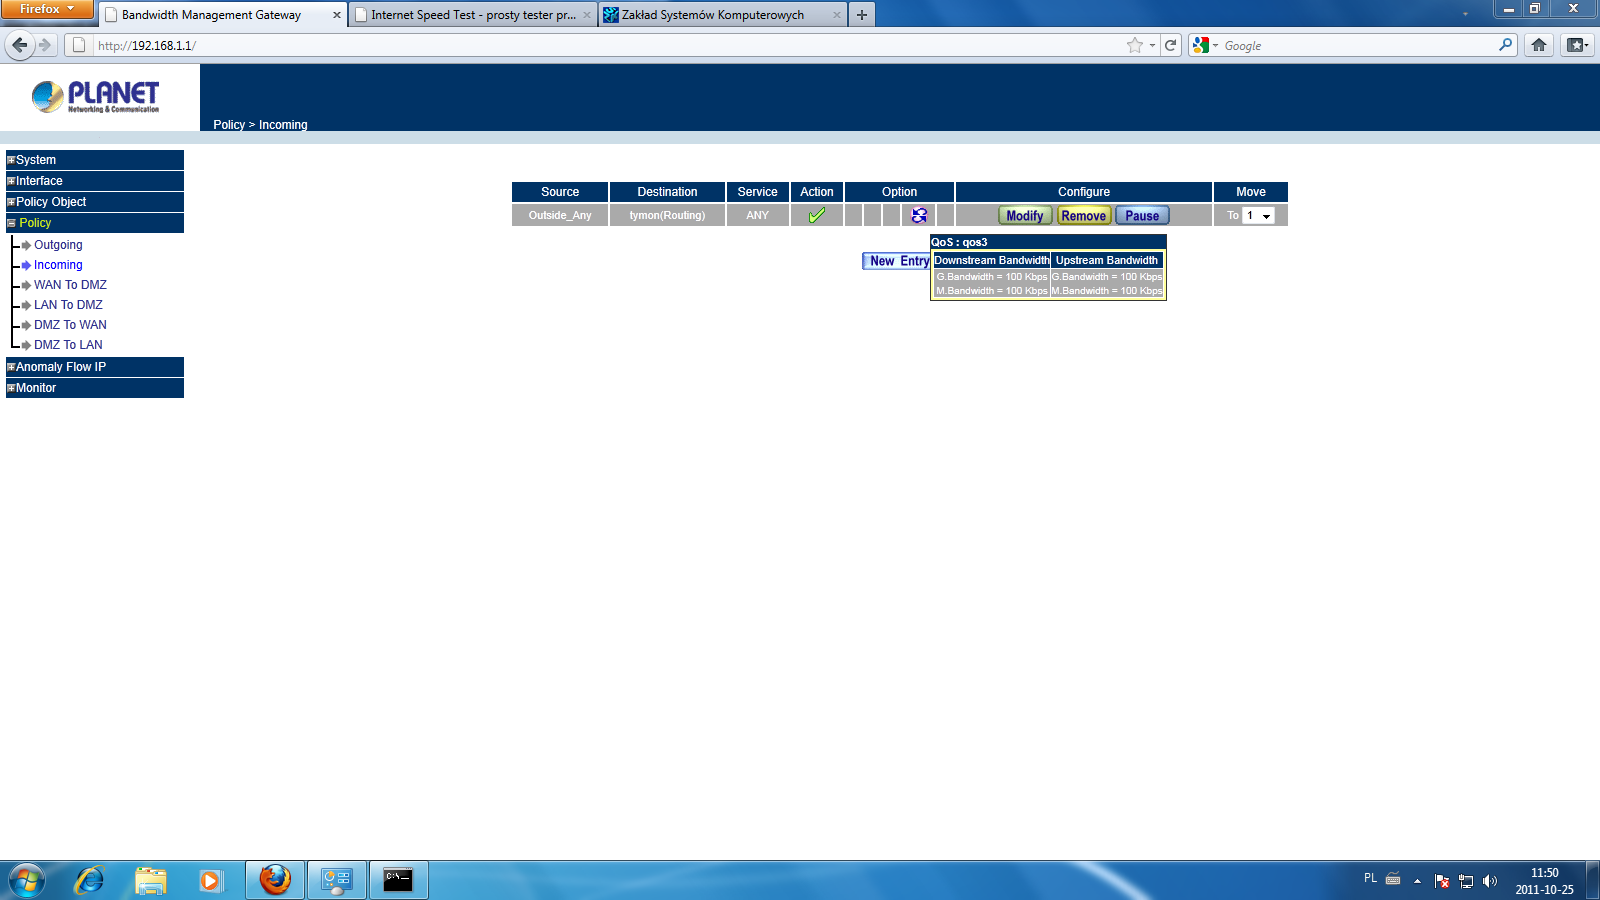
\includegraphics[width=\textwidth]{6.PNG}
    \end{center}
  \end{figure}

  \paragraph{}
  W celu sprawdzenia limitu pasma został wykorzystany serwis \textbf{http://speedtest.net}.
  \begin{figure}[h!]
    \begin{center}
      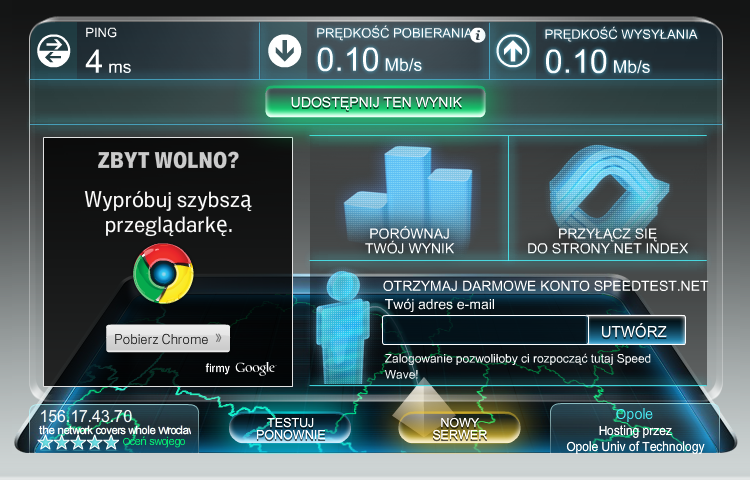
\includegraphics[width=\textwidth]{7.PNG}
    \end{center}
  \end{figure}



  \subsection{Zadanie 7}
  \paragraph{}
  Reguła blokująca pobieranie plików \textbf{.exe}.
  \begin{figure}[h!]
    \begin{center}
      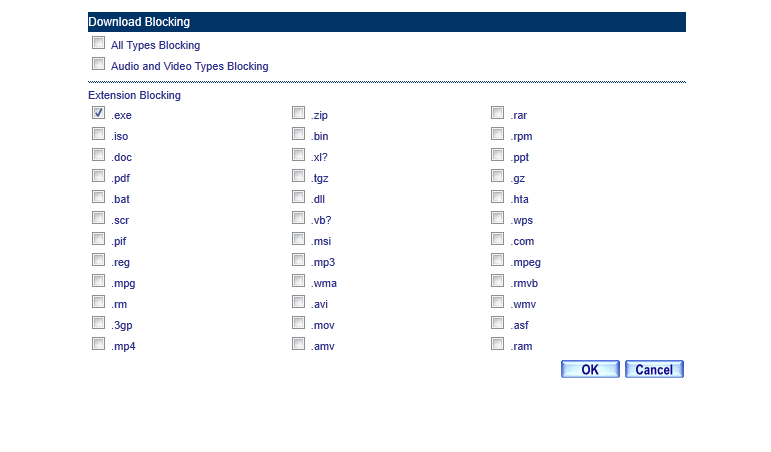
\includegraphics[width=\textwidth]{blocking_exe.PNG}
    \end{center}
  \end{figure}

  \paragraph{}
  Przetestowanie reguły blokującej pobieranie plików \textbf{.exe}.
  \begin{figure}[h!]
    \begin{center}
      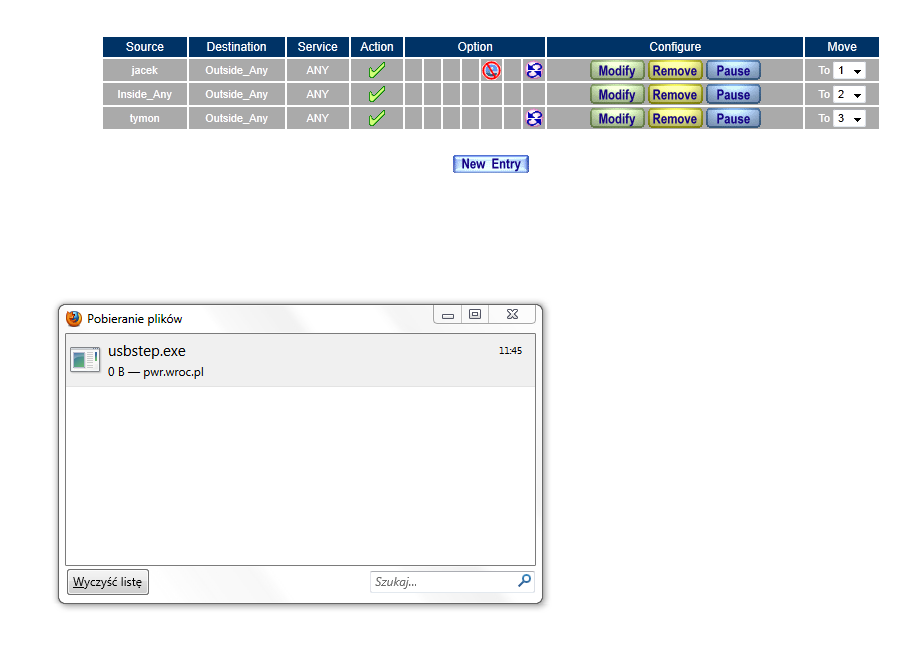
\includegraphics[width=\textwidth]{pobieranie_exe.PNG}
    \end{center}
  \end{figure}



  \subsection{Zadanie 8}
  \paragraph{}
  Reguła umożliwiająca połączenie jedynie ze stroną \textbf{kssk.pwr.wroc.pl}.
  \begin{figure}[h!]
    \begin{center}
      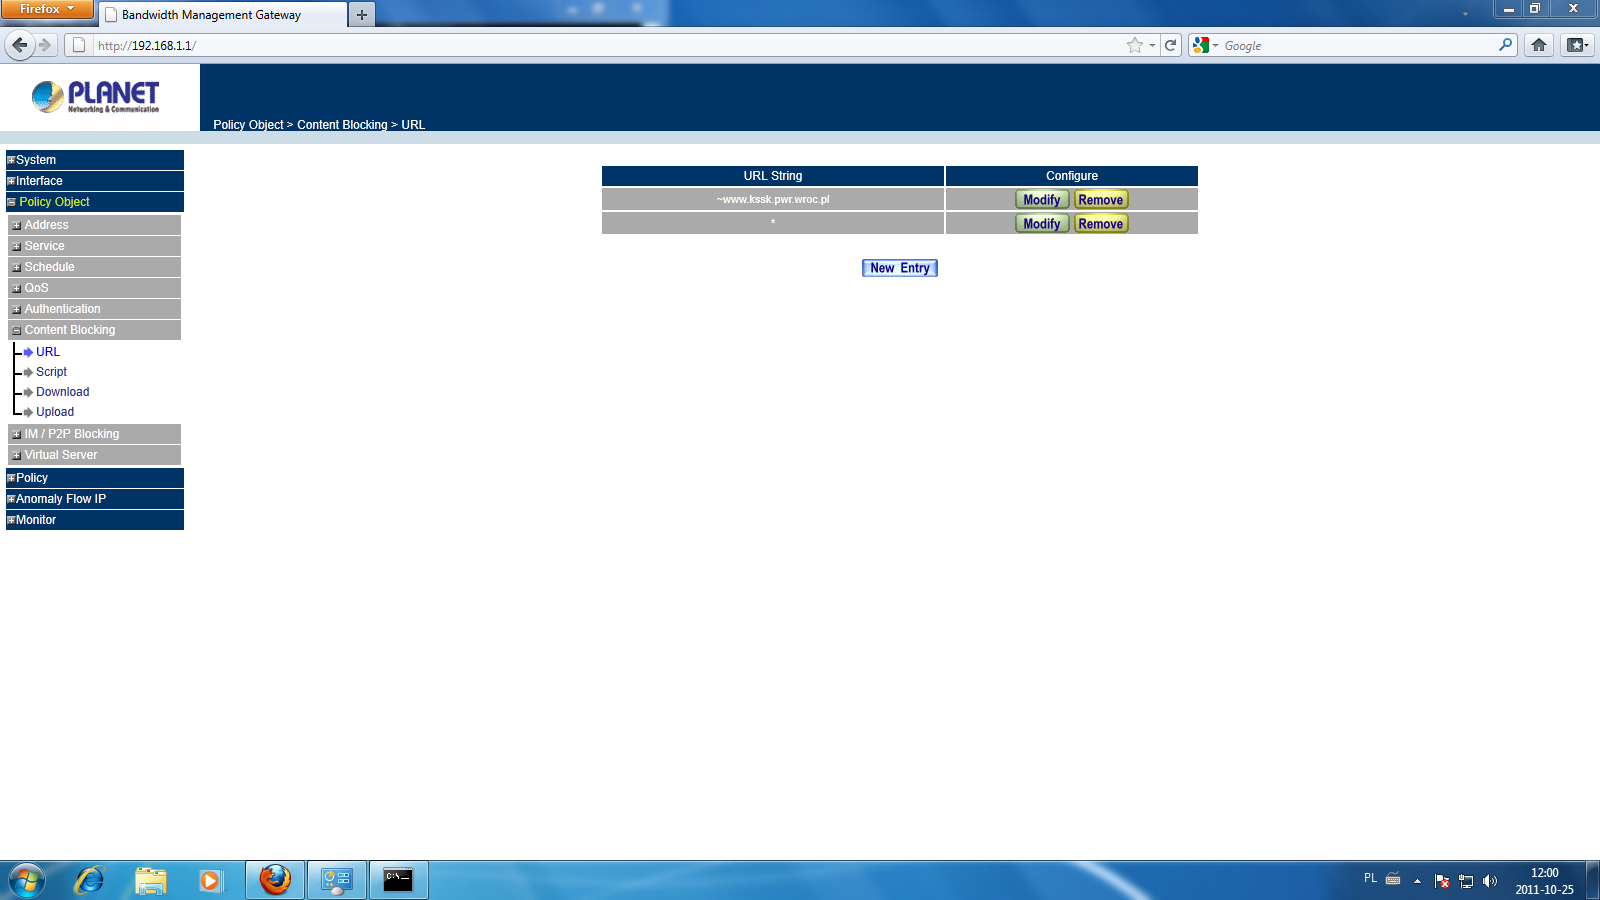
\includegraphics[width=\textwidth]{8.PNG}
    \end{center}
  \end{figure}


  \subsection{Zadanie 9}
  \paragraph{}
  Statystyki ruchu w sieci
  \begin{figure}[h!]
    \begin{center}
      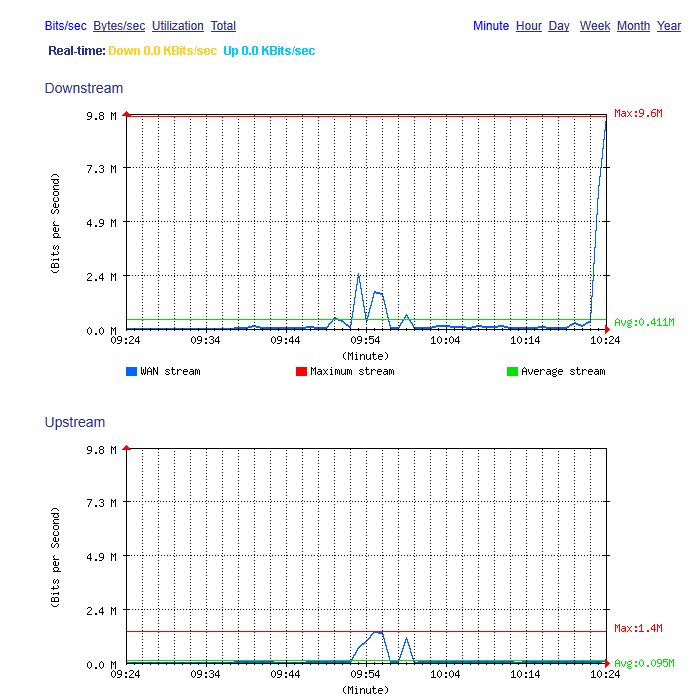
\includegraphics[width=\textwidth]{9.PNG}
    \end{center}
  \end{figure}


  \subsection{Zadanie 10}
  \paragraph{}
  Czasowe blokowanie domen.
  \begin{figure}[h!]
    \begin{center}
      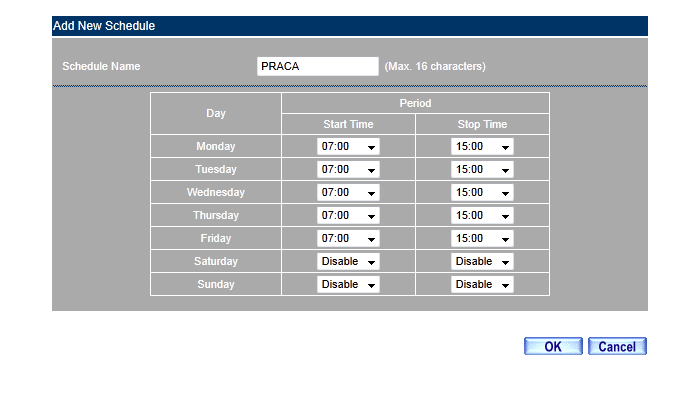
\includegraphics[width=\textwidth]{10.PNG}
    \end{center}
  \end{figure}
  \begin{figure}[h!]
    \begin{center}
      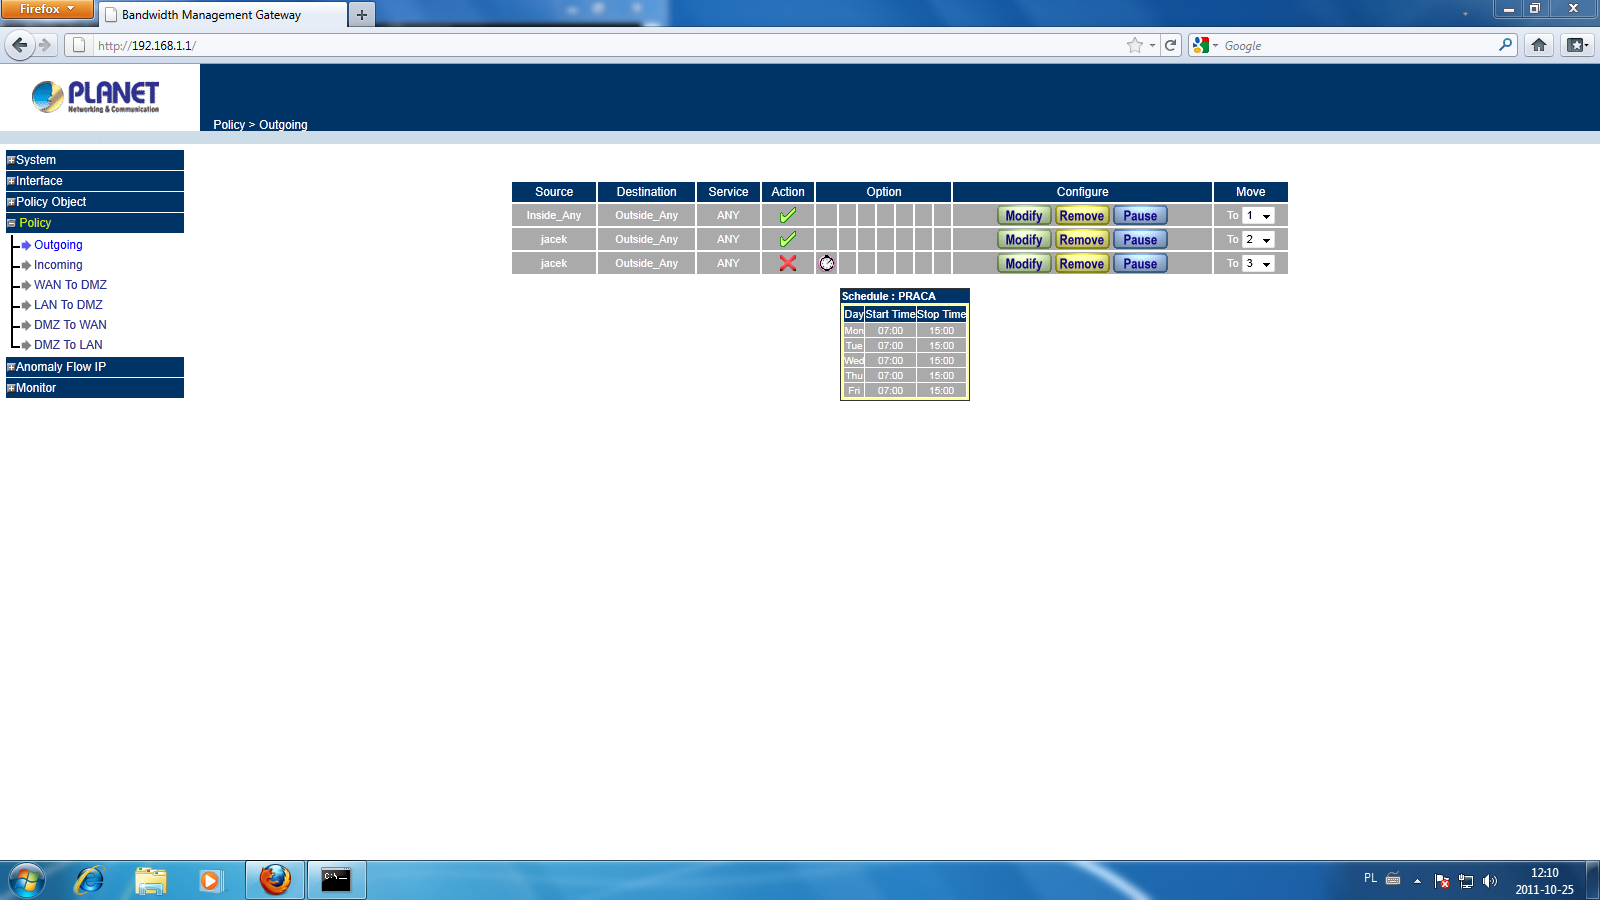
\includegraphics[width=\textwidth]{11.PNG}
    \end{center}
  \end{figure}

  \subsection{Zadanie 11}
  \paragraph{}
  Eksport ustawień routera do pliku.
  \begin{figure}[h!]
    \begin{center}
      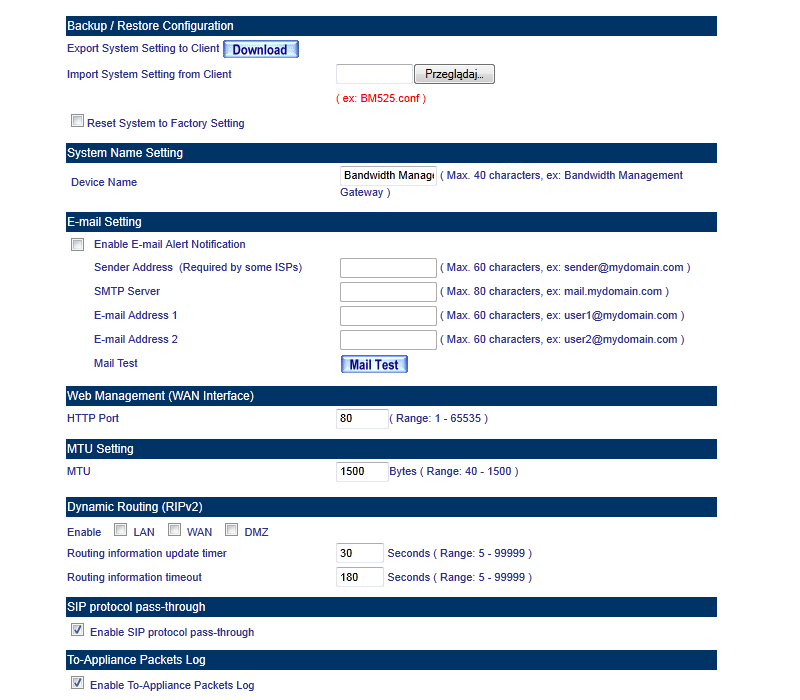
\includegraphics[width=\textwidth]{12.PNG}
    \end{center}
  \end{figure}


  \subsection{Zadanie 12}
  \paragraph{}
  Ustawienie automatycznej synchronizacji zegara z serwerem czasu rzeczywistego.
  \begin{figure}[h!]
    \begin{center}
      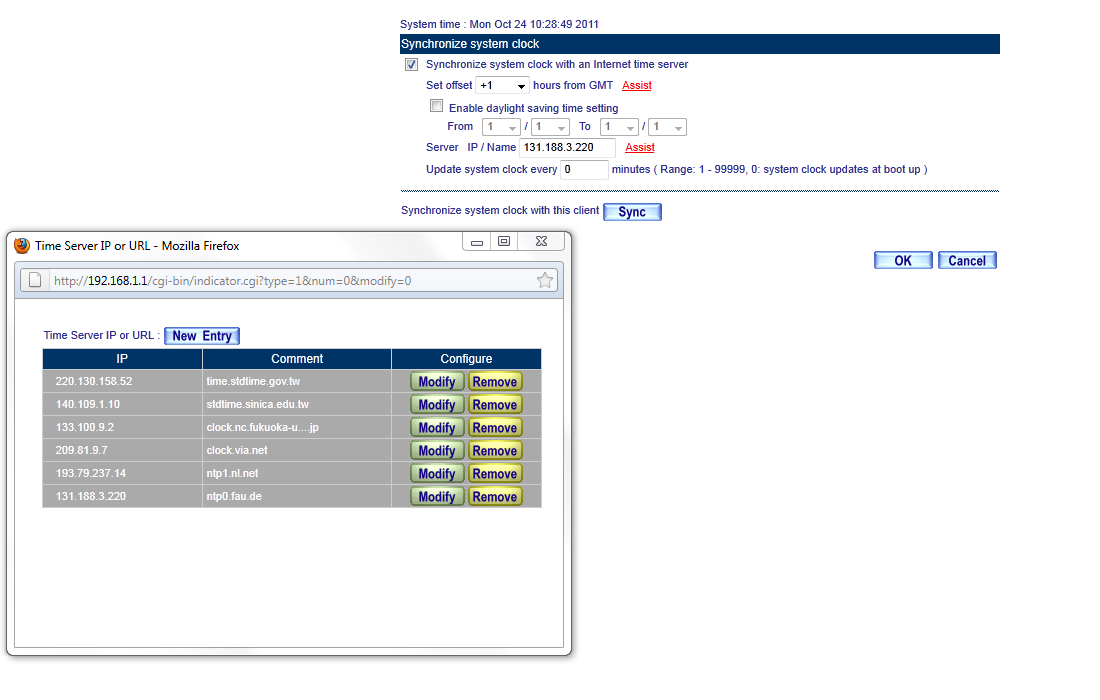
\includegraphics[width=\textwidth]{14.PNG}
    \end{center}
  \end{figure}


  \subsection{Zadanie 13}
  \paragraph{}
  Ustawienie priorytetu dla pakietów różnych usług.
  \begin{figure}[h!]
    \begin{center}
      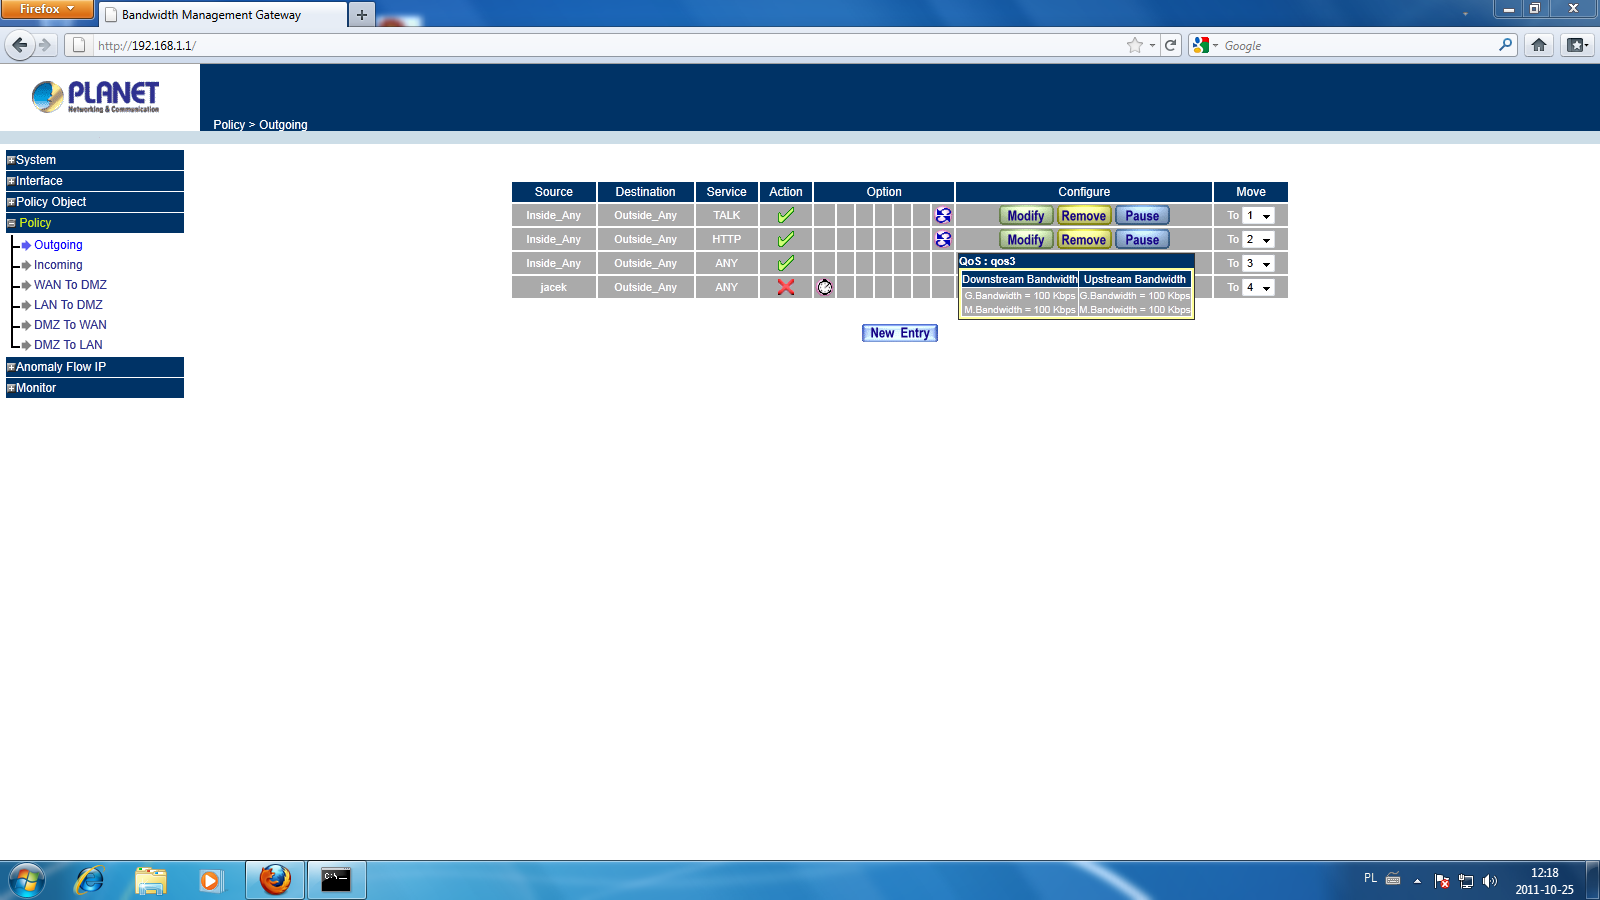
\includegraphics[width=\textwidth]{15.PNG}
    \end{center}
  \end{figure}

  \begin{figure}[h!]
    \begin{center}
      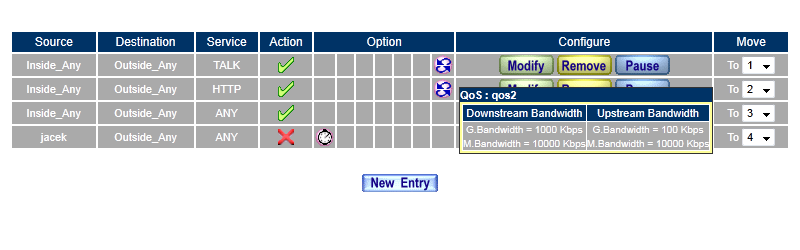
\includegraphics[width=\textwidth]{16.PNG}
    \end{center}
  \end{figure}



  \section{Wnioski}
  \paragraph{}

\end{document}